\section{Dialogue Manager}

The \emph{DM (dialogue manager)} component typically deals with (1) \emph{state tracking}, which refers to representing information from the past as dialogue states; (2) \emph{action selection} or \emph{dialogue strategy}, which refers to mapping from dialogue states to system actions.

Hand-crafting the dialogue strategy in DM can be quite labor intensive. In order to alleviate the painstaking human efforts, several DM architectures and frameworks are proposed, aiming to allow rapid development of dialog management components for spoken dialog systems operating in complex, goal-oriented domains \cite{Bohus2003,Rudnicky1999a}

Two more sophistigated and successful approaches for strategy learning are \emph{Markov decision process (MDP)} \cite{Levin2000A} and \emph{partially observable Markov decision process (POMDP)} \cite{Young2013Pomdp, Gasic2011}. MDP learns to map dialogue states to actions and does not model the uncertainty about states. To tackle the problem, POMDP maintains a distribution over dialogue, i.e. \emph{belief state}, and based on the distribution actions are chosen. Both MDP and PMDMP methods need to learn in an interactive manner. Schatzmann et al. present a survey of the simulated users \cite{Schatzmann2006}, which are commonly used to create the interactive environment.

The far-reaching deep learning techniques are also significantly influencing the DM research. Williams et. al propose to automatically infer state representation using neural networks \cite{Williams2016End}. Similarly, several other end-to-end systems reach promising performance without hand-crafted features for dialogue states \cite{Bordes2016Learning}. Recurrent neural networks are used to learn how to update the state in a data-driven manner \cite{Henderson2014Word}. Dhingra et al. present a method that combines the reinforcement technique with deep learning \cite{Dhingra2016End}, which is used to built a dialogue agent that provides users with an entity from a knowledge base.

\subsection{RavenClaw: Dialog Management Using Hierarchical Task Decomposition and an Expectation Agenda \cite{Bohus2003}}

This paper describes \emph{RavenClaw}, a new dialog management framework used in the \emph{CMU Communicator}. RavenClaw introduces a clear separation between task and discourse behaviour specification, and allows rapid development of dialog management components for spoken dialog systems operating in complex, goal-oriented domains.

Dialog management maintains continuity over turns in a conversation between human and computer. The authors believe that the essence of dialog management resides in performing two functions: interpreting user inputs with respect to tasks within the domain, and maintaining the coherence over time. Based on this philosophy, the proposed RavenClaw is a two-tier architecture (cf. Figure \ref{fig:raven_arch}). The \emph{Dialog Task Specification} layer captures all the domain-specific dialog logic. The \emph{Dialog Engine} is a domain-independent component that controls the dialog and contributes basic conversational strategies (e.g., timing and turn-taking behaviour, grounding behaviour, etc.).

\begin{figure}[h]
  \centering
  % Requires \usepackage{graphicx}
  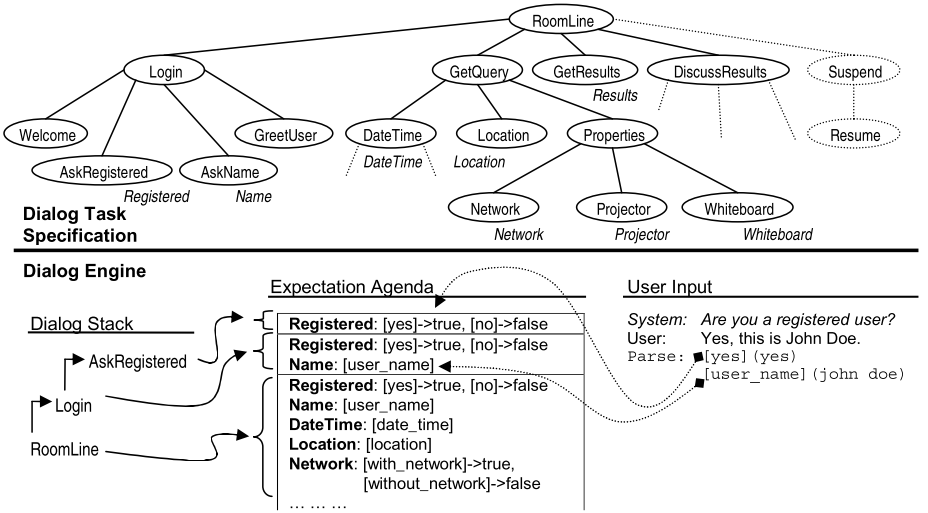
\includegraphics[width=\linewidth]{ravenclaw_arch.png}\\
  \caption{RavenClaw architecture.}\label{fig:raven_arch}
\end{figure}

The domain-specific dialog control is represented in the Dialog Task Specification level using a tree of dialog agents, with each agent handling a certain part of the dialog task. The proposed architecture uses hierarchical task decompositions, which are traditionally used for task execution in robotics. Two categories of dialog agents populate the task tree: \emph{fundamental dialog agents} and \emph{dialog agencies}. The fundamental dialog agents appear as leaf nodes (e.g. \textbf{Welcome}, \textbf{AskRegistered}) and represent atomic dialog actions. The non-terminal nodes in the tree are dialog agencies (e.g. \textbf{Login}, \textbf{GetQuery}), which control the execution of their subsumed agents, capturing the higher level temporal and logical structure of the dialog task.

The Dialog Engine is the core component in RavenClaw and controls the dialog by executing the Dialog Task Specification. Dialog flow is generated by interleaving \emph{Execution Phases} and \emph{Input Phases}. In an Execution Phase, the various agents in the task tree are executed and generate the system's behaviour. In an Input Phase, the system collects and incorporates the information from the user's input.

A characteristic which greatly influences the usability and ultimately the success of spoken dialog systems is their ability to employ a rich set of conversational strategies. These encompass grounding behaviours (e.g. confirmations, disambiguations, etc.), turn-taking and timing behaviours. RavenClaw provides automatic support for all the above mentioned conversational strategies. Internally, they are implemented as dialog agencies, in the same manner as the domain-specific dialog task tree.

Finally, the paper presents five systems using RavenClaw-based dialog managers (LARRI, the Intelligent Procedure Assistant, BusLine, RoomLine and TeamTalk). These implemented systems show that the proposed framework can be easily adapted to different domains, indicating that RavenClaw is with a high degree of versatility and scalability.

\subsection{An Agenda-based Dialog Management Architecture for Spoken Language Systems \cite{Rudnicky1999a}}

This paper proposes a dialog management architecture based on the elements of \emph{handlers}, a \emph{product} and an \emph{agenda}. The goal is to develop a dialog management that can solve two specific problems: 1) providing a coherent coverall structure to interaction that extends beyond the single turn; 2) correctly manage mixed-initiative interaction.

When the paper was written there were two commonly used dialog management approaches: \emph{graph-flow based} systems and \emph{frame-based} systems. Graph-based systems handle the dialog by explicitly enumerating all possible dialog states, as well as allowable transitions between states. However, graph systems have a number of limitations, such as making it difficult for a user to change topic. The frame-based method does not necessarily extend to more complex tasks, for example ones where the goal is to create a complex data object, such as a plan.

The paper first describes a \emph{script-based dialog manager}, before formally introducing the more sophisticated agenda-based architecture. Script in the context simply refers to an explicit sequencing of task-related topics. Each topic is expressed as a form-filling task. In the control strategy, slots are pre-ordered based on their ability to constrain the solution; this ordering provides a default sequence in which the system selects to ask the user about. Figure \ref{fig:R99a-script_based} shows the structure of the Flight Leg topic in the script-based system.

\begin{figure}[h]
  \centering
  % Requires \usepackage{graphicx}
  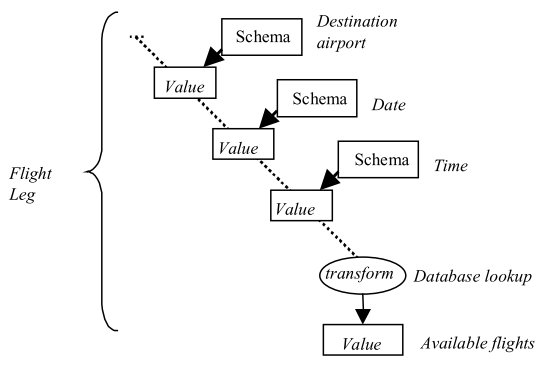
\includegraphics[width=.6\linewidth]{R99a-script_based.png}\\
  \caption{Task-based dialog control in a script-based system.}\label{fig:R99a-script_based}
\end{figure}

The script-based approach still has a number of limitation, such as making it difficult to navigate over the product. So the paper further proposes an \emph{agenda-based} architecture.

The proposed architecture introduces two new data structures: an \emph{agenda} to replace a fixed script, and a \emph{dynamic product} that could evolve over the course of a session. In the agenda-based system, the product is represented as a tree, which reflects the natural hierarchy and order of the information needed. A dynamic product is simply one that can be modified over the course of a session.

Operationally, this means providing a set of operators over tree structures and making these available to the user and to the system. Each node in the product tree corresponds to a handler, which encapsulates computation relevant to a single information item. The agenda is an ordered list of topics, represented by handlers that govern some single item or some collection of information. The agenda specifies the overall ``plan'' for carrying out a task.
The handler on the top of the agenda has the highest priority and represents the focused topic. When a user input comes in, the system calls each handler per their order in the agenda, and each handler will try to interpret the user input and generate the response.

The proposed dialog management architecture is implemented in the \emph{CMU Communicator} system, which handles a complex travel task consisting of air travel, hotels and car reservations. The system uses the \emph{Sphinx II} speech recognizor in a real-time mode and supports barge-in. A top-1 hypothesis is produced by the decoder and parsed by \emph{Phoenix} using a semantic domain-specific grammar. The example dialog presented in the paper shows a number of features of the proposed architecture: the ability to absorb implicit changes of topic on the part of the user, adding to an existing itinerary, and handling explicit topic shifts.

\subsection{A stochastic model of human-machine interaction for learning dialog strategies \cite{Levin2000A}}

This paper proposes a quantitative model for dialog systems that can be used for learning the dialog strategy. After formalising the dialog design as a \emph{Markov decision process (MDP)}, the reinforcement learning algorithm is used to find the optimal strategy. This approach is evaluated in an \emph{air travel information system (ATIS)} task.

The key idea of this paper is to formalise the dialog design as an optimization problem with an objective function reflecting different dialog dimensions for a given application. With some assumptions about the state transition probabilities and cost assignment, a dialog system can be mapped to a MDP, which has a variety of data driven algorithms for finding the optimal strategy.

The first step is to state the problem of dialog design as optimization of an objective $C$:
$$C = \sum W_i \langle C_i \rangle,$$
where the terms $\langle C_i \rangle$ are the expected costs for different dialog dimensions. The paper illustrates the concepts with a toy example of ``Day-and-Month Dialog'', where the goal is to get the correct day and month values from the user. In the case, the objective $C$ has three components: the first part denotes the \emph{expected duration} of the dialog; the second part denotes the expected number of error; the last part corresponds to the expected distance from achieving the application goal. With this concept, the goal of a dialog system is to minimize the cost function.

\begin{figure}[htbp]
  \centering
  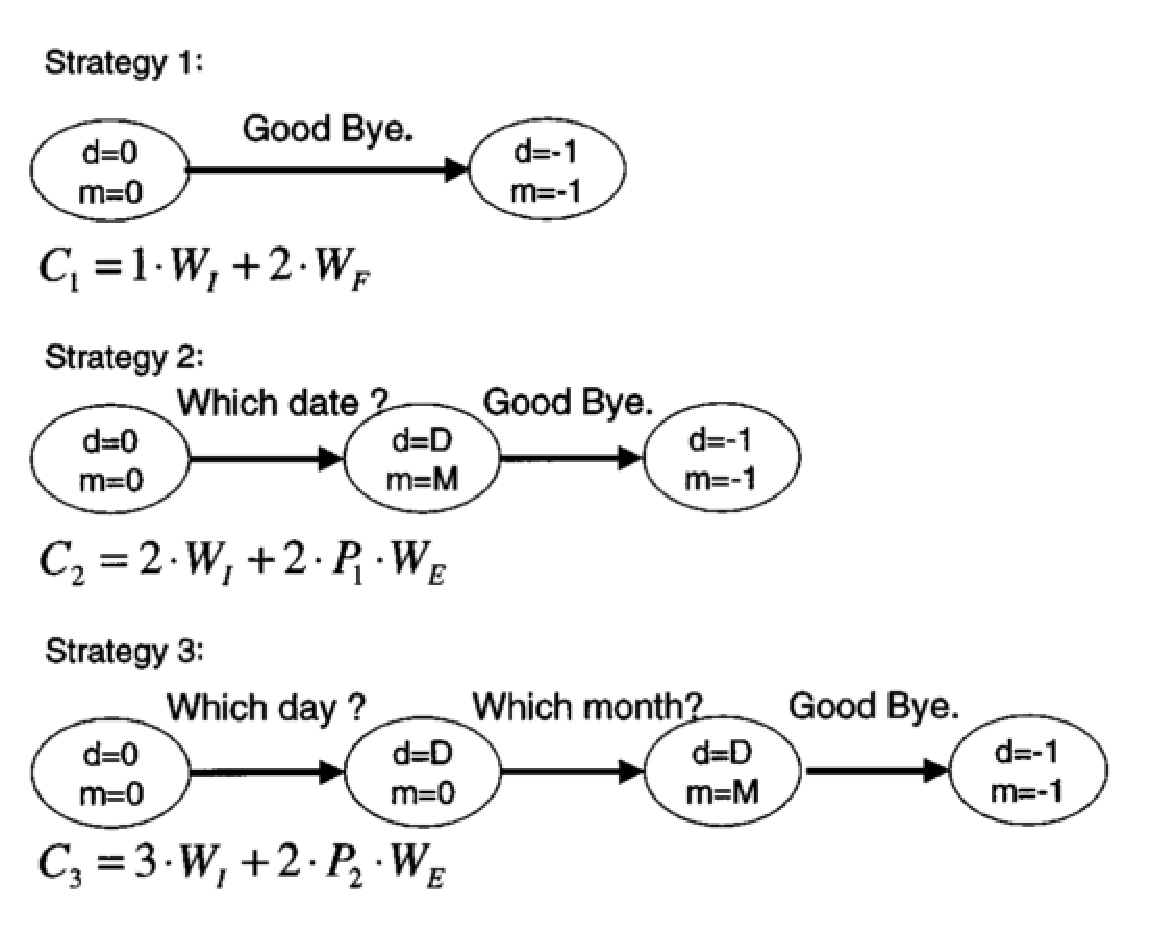
\includegraphics[width=.6\linewidth]{10_17_dialog_MDP1}\\
  \caption{Three possible strategies for the day-month dialog system}\label{fig:dialog_MDP1}
\end{figure}

The next step is to formalize a dialog system as a sequential decision process in terms of its action set, state space, and strategies: 1) The action set of the dialog system includes all possible actions it can perform, such as interactions with the user (e.g., asking the user for input, providing some output, etc.). In the toy example, there are four actions, such as asking for the day $A_d$, asking the month $A_m$, asking the date (day and month) $A_{dm}$, and a final action $A_f$; 2) The state $s$ includes the values of all relevant variables that determine the next action. In the example each state has two integer variables, $d \in \{0, ..., 31\}$ and $m \in \{0, ..., 12\}$, corresponding to the day and month respectively. 3) A dialog strategy maps each state to an action. For example, Figure \ref{fig:dialog_MDP1} shows three possible strategies for the example system.

With some assumptions about the transition probabilities between states, and the cost assignment, the sequential decision process can be formalise as a MDP. Then the optimal strategy can be obtained by a variety of reinforcement learning algorithms.

However, in reinforcement learning, the optimal strategy is learned not from a static corpus but through interaction, because the strategy itself determines the distribution of states in the corpus. To overcome this problem, the paper proposes the use of a \emph{simulated user}. The simulated user is a stochastic generative model that produces speech acts as a response to a dialog action. The simulated user does not deal with the language understanding component - it communicates with the dialog system through semantic representations. The parameters of the simulated user can be estimated from an annotated dialog corpus.

\begin{figure}[htbp]
  \centering
  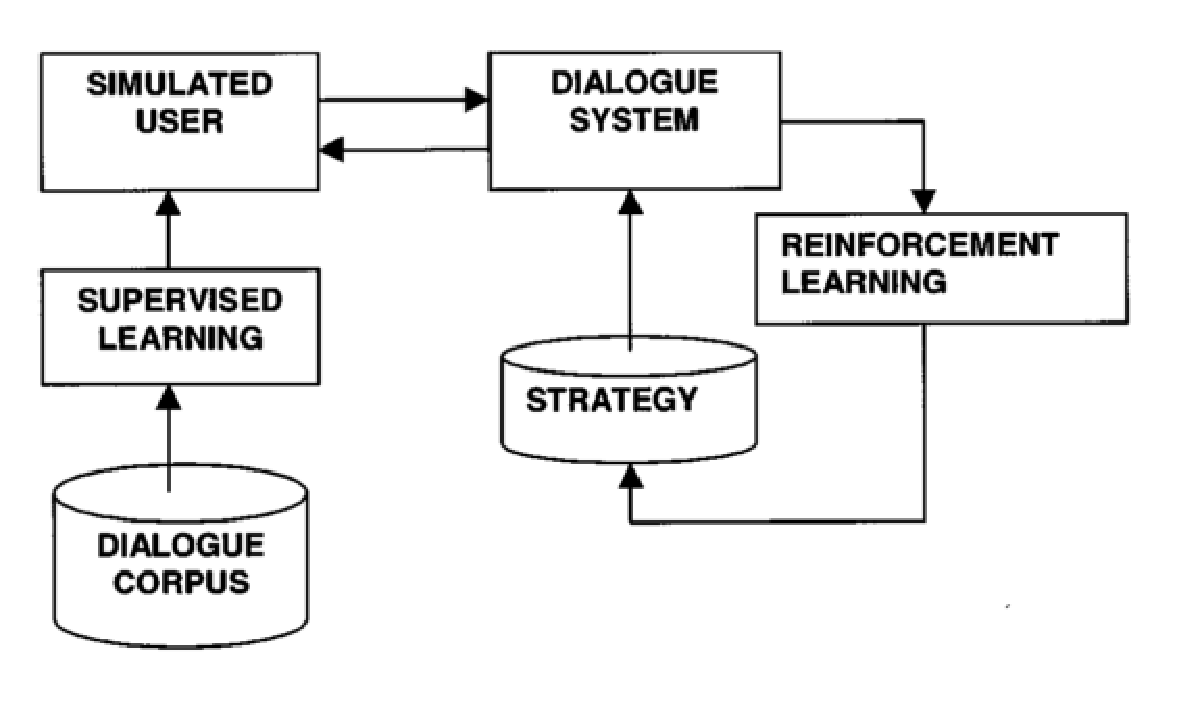
\includegraphics[width=.6\linewidth]{10_17_dialog_MDP2}\\
  \caption{Procedural description of the learning paradigm}\label{fig:dialog_MDP2}
\end{figure}

Once a simulated user is available, it can be used in a generative mode for interacting with the dialog system while the reinforcement learning algorithm is estimating the optimal strategy. Then when a reasonable estimate of the optimal strategy is obtained, the system can be used with real users and the learning process can continue. Figure \ref{fig:dialog_MDP2} summarizes the suggested learning paradigm.

\begin{figure}[htbp]
  \centering
  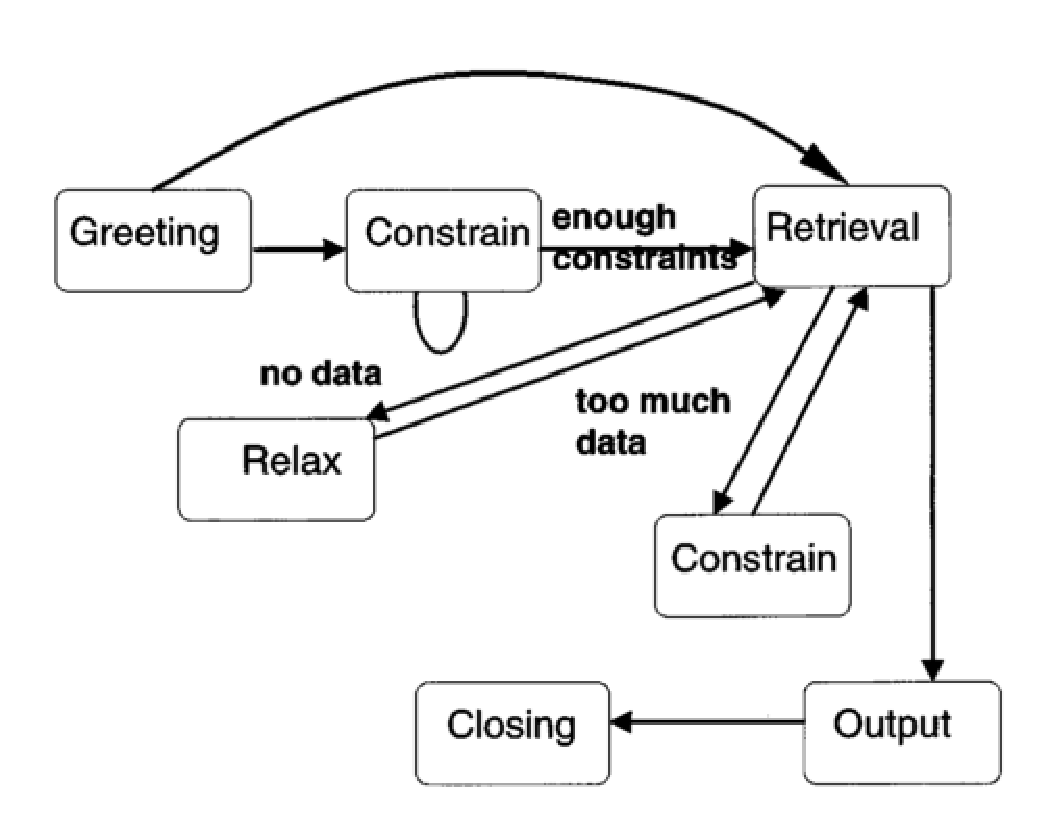
\includegraphics[width=.5\linewidth]{10_17_dialog_MDP3}\\
  \caption{Schematic representation of the optimal strategy for ATIS}\label{fig:dialog_MDP3}
\end{figure}

In the experimental study, the paper shows that a nontrivial strategy can be automatically learned given the simple objective function. For example, Figure \ref{fig:dialog_MDP3} shows the learned strategy of the ATIS task.

Remark: I have also considered formalising the dialog manager as a MDP, and realised one obvious difficulty is that there is not an interactive environment to train the system. This paper introduces simulated users to overcome this difficulty. Another good idea is to abstract the dialog process, such as using semantic representations without considering the ASR or NLU component. I think this paper shows a very promising approach for building our chatbot. 
\subsection{POMDP-based Statistical Spoken Dialogue Systems: a Review \cite{Young2013Pomdp}}

By including an explicit Bayesian model of uncertainty and by optimising the policy via a reward-driven process, \emph{partially observable Markov decision processes (POMDPs)} provide a data-driven framework that reduces the cost of hand-crafting dialog managers and provides robustness against the errors created by speech recognisers operating in noisy environments. This paper provides an overview of the current state of the art in the development of \emph{POMDP-based spoken dialog systems (SDS)}.

\begin{figure}[htbp]
  \centering
  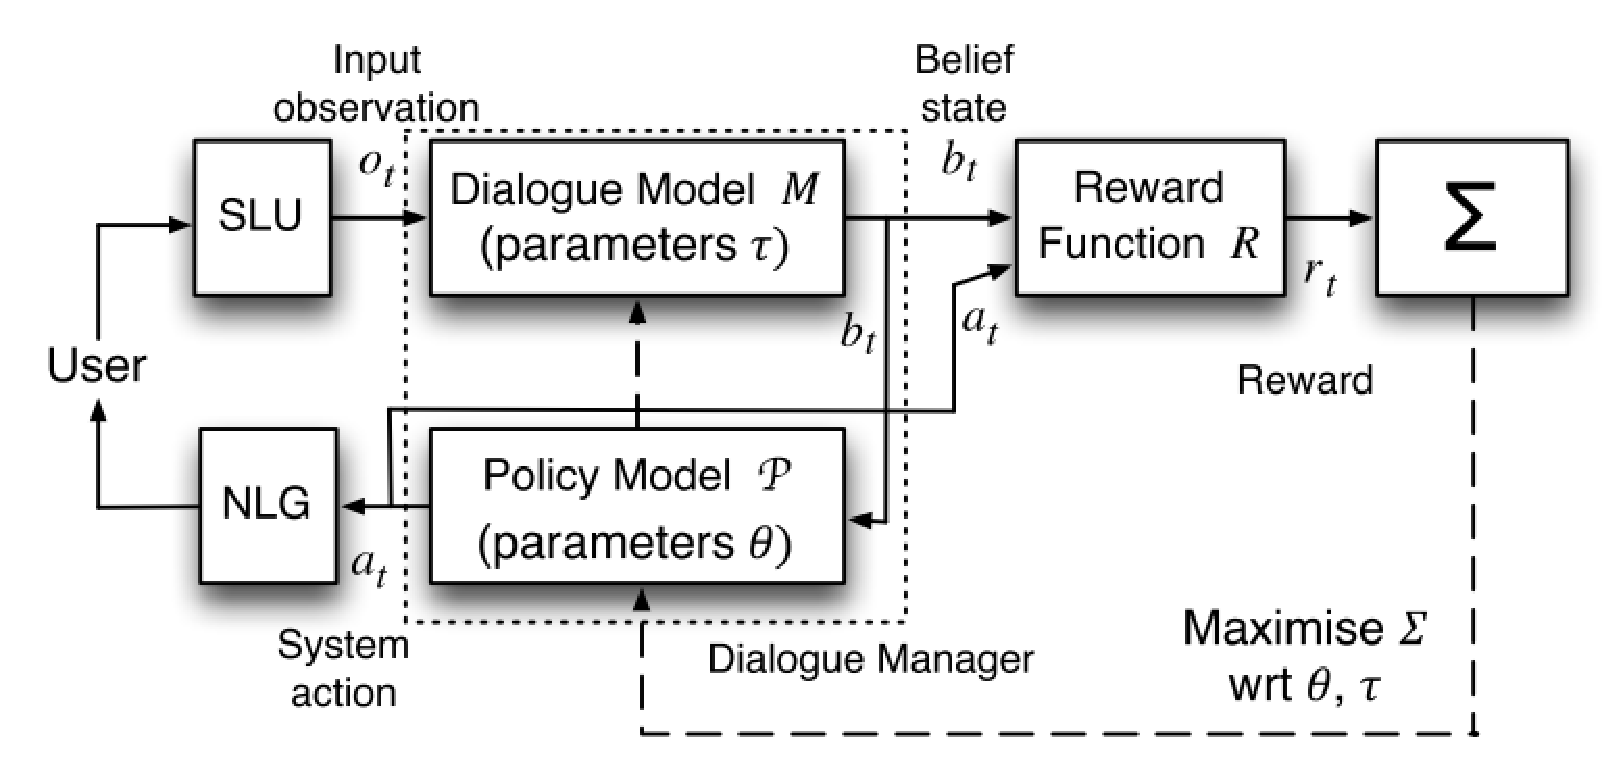
\includegraphics[width=.7\linewidth]{10_17_POMDP1}\\
  \caption{Components of a POMDP-based spoken dialog system}\label{fig:POMDP1}
\end{figure}

%The principal elements of a conventional Spoken Dialog System (SDS) are shown in Figure \ref.
The POMDP approach assumes that dialog evolves as a Markov process, i.e., starting in some initial state, each subsequent state is modelled by a transition probability $p(s_t | s_{t-1}, a_{t-1})$. The state $s_t$ is not directly observable. At each turn, the system regards the output of the SLU as a noisy observation $o_t$ of the user input with probability $p(o_t | s_t)$. The transition and observation probability functions are represented by the dialog model. The decision as to which action to take is represented by the policy. The components of a POMDP-based system are presented in Figure \ref{fig:POMDP1}.

\begin{figure}[htbp]
  \centering
  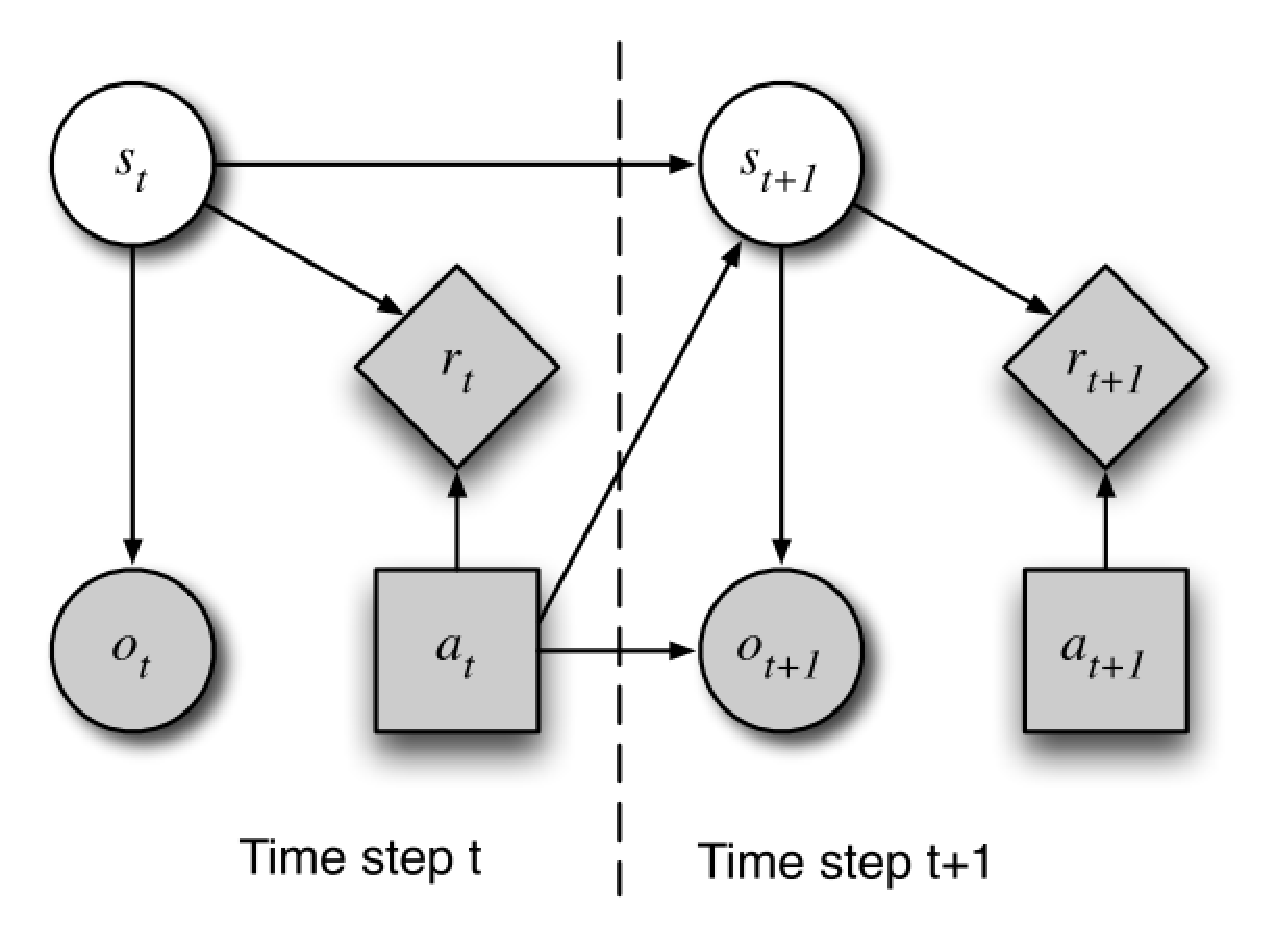
\includegraphics[width=.5\linewidth]{10_17_POMDP2}\\
  \caption{An influence diagram of a POMDP}\label{fig:POMDP2}
\end{figure}

The paper first introduces some preliminary knowledge about the POMDP method. In a POMDP system in each step the world is in some unobserved state $s_t$. Since $s_t$ is not known exactly, a distribution over possible states called a belief state $b_t$ is maintained, where $b_t(s_t)$ indicates the probability of being in a particular state $s_t$. Based on $b_t$, the machine selects an action $a_t$, receives a reward $r_t$, and transitions to (unobserved) state $s_{t+1}$. The machine then receives an observation $o_{t+1}$. This process is represented as an influence diagram in Figure \ref{fig:POMDP2}.

Given an existing belief state $b_t$, the last system action $a_t$, and a new observation $o_{t+1}$, the new updated belief state is given by:
$$b_{t+1}(s_{t+1}) = \eta P(o_{t+1} | s_{t+1}, a_t) \sum_{s_t} P(s_{t+1} | s_t, a_t)  b_t(s_t),$$
where $\eta$ is a normalization constant. The system action is determined by a policy $\pi$. The discounted sum of rewards expected by starting in $b_t$ and following policy $\pi$ is given by the value function $V^\pi(b_t)$. In POMDP, finding an optimal policy is called solving or optimizing the POMDP. However, standard POMDP methods do not scale to the complexity needed to represent a real-world dialog system. So the next sections of this paper introduce some domain-specific methods for applying POMDP in the SDS task.

The first step is to review some possible approaches to represent the dialog model. In a goal-oriented SDS, the state should encode three distinct types of information: the user's goal $g_t$, the intent of the most recent user utterance $u_t$, and the dialog history $h_t$. The resulting influence diagram is shown in Figure \ref{fig:POMDP2}, in which some reasonable independence assumptions have been introduced. Factoring the state in this way can significantly reduce the POMDP model complexity. However, it is still too complex to support tractable real-world systems, so further approximation is necessary. The paper introduces two main approaches: the N-best approach, and the factored Bayesian Network approach.

In N-best approaches, the belief state is approximated by a list of the most likely states with their probabilities. It can also be viewed as running N conventional dialog systems in parallel, such that each parallel thread tracks a different interpretation of what the user said.

\begin{figure}[htbp]
  \centering
  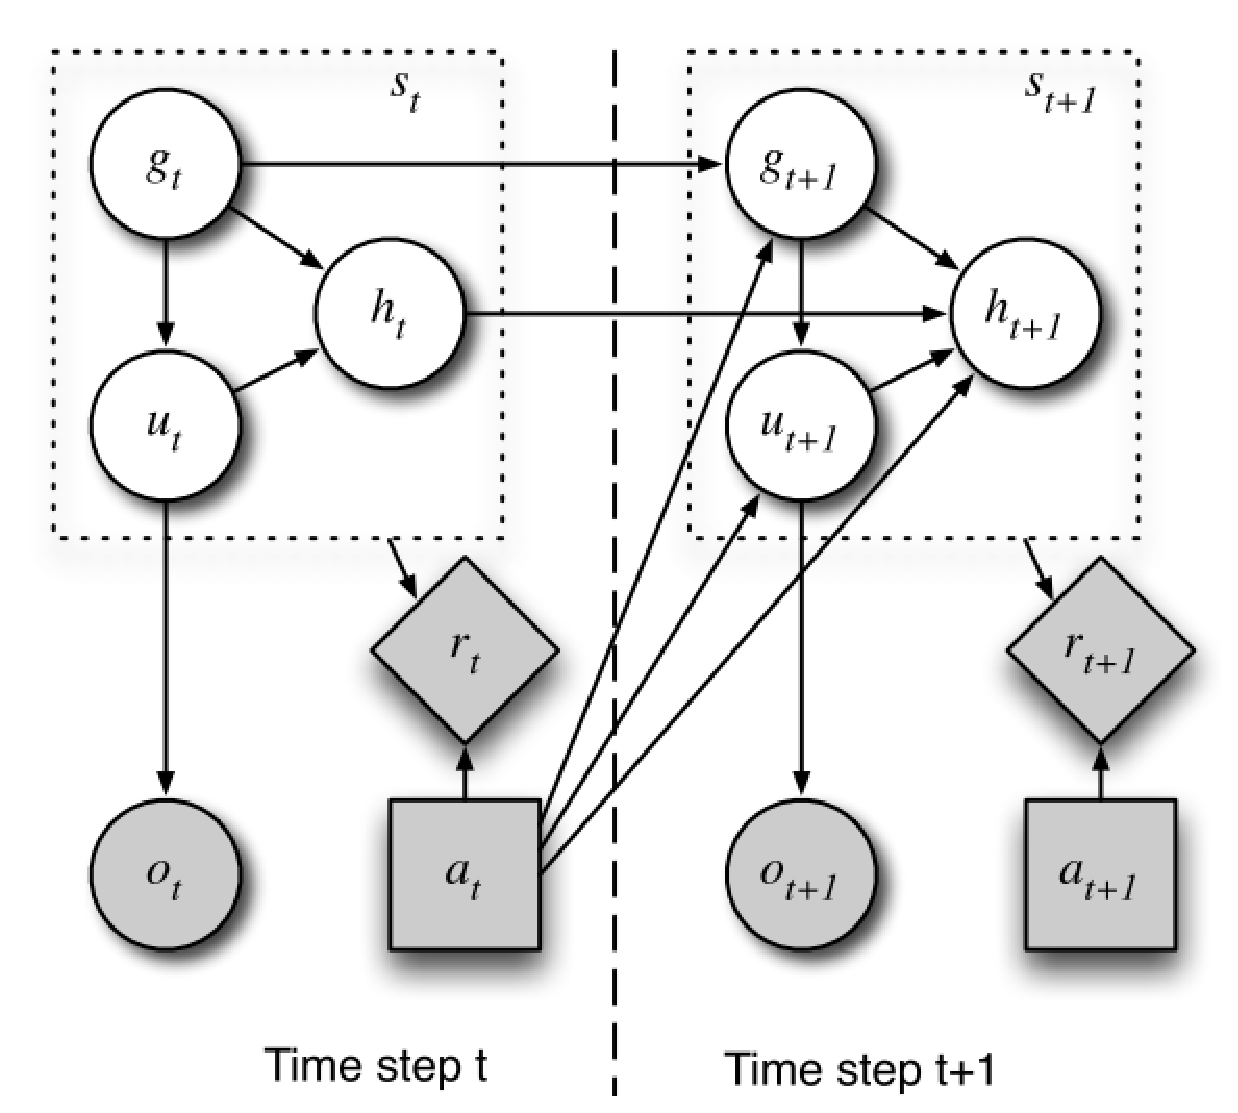
\includegraphics[width=.5\linewidth]{10_17_POMDP3}\\
  \caption{An influence diagram of a factored state POMDP}\label{fig:POMDP3}
\end{figure}

The second approach is to factor the user goal into concepts that can be spoken about by the system. This is illustrated in Figure \ref{fig:POMDP3}, which shows an example from a tourist information system, in which entities have a type, the kind of food served and an area.

The next big challenge of a POMDP-based system is the representation and estimation of the policy model. The paper presents five different methods of policy optimisation: planning under uncertainty, value iteration, Monte-Carlo optimisation, least-squares policy iteration, and natural actor-critic. These methods have been selected because all have been applied to end-to-end working dialog systems.

Another problem is also mentioned in the previous paper summaries of the MDP-based approaches: learning directly from corpora is problematic, because an interactive environment is necessary. One solution is to build a model of the user that can interact directly with a dialog system, and which can itself be trained on corpora. In a real system the dialog manager only has access to a noisy observation, so an error model is needed as well as a user model.

The following three sections presents some more advanced techniques for dialogue model parameter optimisation, fast training, user adaption, and discusses some real-world systems and applications. Finally, the paper discusses the current evaluation methods of SDS. Evaluation of SDS typically falls into one of 3 testing regimes: testing with some form of simulated user, testing with paid subjects, and testing within a live deployed system.

Remark: I am not very familiar with the POMDP approach, so some of the technical details mentioned in the paper are still not very clear to me. Intuitively, POMDP should have better performance than MDP (but also harder to train). I think it is also possible to combine it with the deep learning techniques, such as representing the transition probabilities with a neural network approximately. 
\subsection{On-line policy optimisation of Bayesian spoken dialogue systems via human interaction \cite{Gasic2011}.}

The task is to learn system policy, which determines system acts based on dialouge states (see Table \ref{Goal-Oriented Dialogue System Example} for an example). The paper applies GP-Sarsa to automatic policy learning, which is an online RL algorithms based on Gaussian process \cite{Engel2014Reinforcement}. The GP-Sarsa optimization adopts a more robust filtered reward function \cite{Gasic2011}.

\subsection{A Survey of Statistical User Simulation Techniques for Reinforcement-Learning of Dialogue Management Strategies \cite{Schatzmann2006}}

This paper briefly summarizes the role of the dialogue manager in a \emph{Spoken Dialogue System (SDS)}, gives a short introduction to reinforcement-learning of dialogue management strategies and reviews the literatures on user modelling for simulation-based strategy learning. It further describes recent work on user model evaluation and discusses some of the current research issues.
\begin{figure}[h]
  \centering
  % Requires \usepackage{graphicx}
  \includegraphics[width=.6\linewidth]{khan2004-dm.png}\\
  \caption{learning dialogue strategies with a simulated user}\label{fig:khan04-dm}
\end{figure}

In SDS, the task of the \emph{dialogue Manager (DM)} is to control the flow of the dialogue and to decide which actions to take in response to user input. Specifically, DM needs a \emph{dialogue strategy} that defines when to take the initiative, when to confirm receipt, and so forth. An interesting approach to learn such strategies is through training a statistical, predictive user model for simulating user responses, which can then be used to learn the desired dialogue strategies through trial-and-error interactions (cf. Figure \ref{fig:khan04-dm}).

The second and third sections of the paper discuss  the role of the dialogue management and the reinforcement technique. Since these topics are already covered in other relevant summaries, we choose not to present them here.

Compared with the early rule-based approaches for user modelling, statistical user models are more appealing for the following reasons: 1) The purpose of the user model is not to capture the individual characteristics of a specific user, but to form the basis of a user simulation tool, so it needs to represent the statistical distribution over all types of user behaviour and user responses. These requirements clearly favour a statistical approach; 2) The second advantage of statistical models is that the model parameters can be estimated using real human-computer dialogue data. 3) The user model is also likely to be more robust, more scalable and easier to port to a different domain or dataset. The paper then summaries the recent statistical models into the following groups:

\textbf{N-grams} This method introduces a simple n-gram model for predicting the user action $\hat{a}_{u,t}$ at time $t$ that is most probable given the dialogue history of system and user actions. The weakness of the early bigram model is that it does not place any constraints on the simulated user behaviour. The bigram model is modified to predict only ``sensible'' user responses in some later work, but it still doest not ensure consistency over the course of a dialogue, because of the flawed assumption that every user response depends only on the previous system turn.

\begin{figure}[h]
  \centering
  % Requires \usepackage{graphicx}
  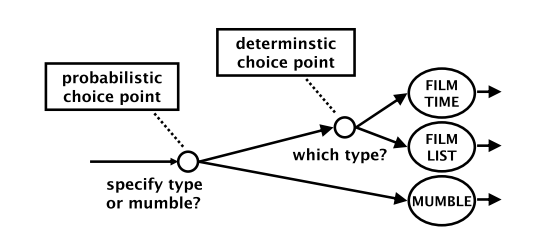
\includegraphics[width=.6\linewidth]{khan2004-graph.png}\\
  \caption{An example of the graph-based approach}\label{fig:khan04-graph}
\end{figure}

\textbf{Graph-based Models} This method combines deterministic rules for goal-dependent actions and probabilistic modelling to cover the conversational behaviour of the simulated user. An example model is shown in Figure \ref{fig:khan04-graph}, in which the arcs of the network represent actions and the nodes represent choice points. Some of the choice points are identified as probabilistic, representing a random decision by the simulated user. The major disadvantage is the high dependence on domain-specific knowledge, and the identification of probabilistic/deterministic choice points requires manual effort.

\begin{figure}[h]
  \centering
  % Requires \usepackage{graphicx}
  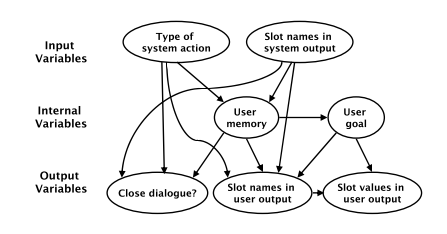
\includegraphics[width=.6\linewidth]{khan2004-bayesian.png}\\
  \caption{An example of the Bayesian Network approach}\label{fig:khan04-bayesian}
\end{figure}


\textbf{Bayesian Networks} The goal of this approach is to avoid the manual effort involved in building networks of choice points, while ensuring that actions are consistent with the user's goal. Figure \ref{fig:khan04-bayesian} shows an example of the network. It is suggested that the network can be easily extended to include factors such as the level of cooperativeness, the degree of initiative, etc.

\textbf{Machine-Learning Techniques} Recent work by Georgila et al. \cite{Georgila2005} returns to Markov models and explores the use of richer state descriptions, longer dialogue histories and machine-learning techniques. They use linear feature combination to map from a state $s$ to a vector of real-valued features $f(s)$. Supervised learning is then used to estimate a set of weights which describe how useful each vector element of $f(s)$ is for predicting an action $a$.

\begin{figure}[h]
  \centering
  % Requires \usepackage{graphicx}
  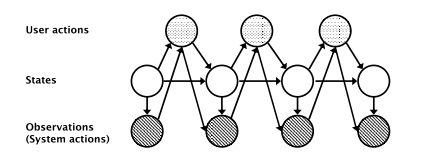
\includegraphics[width=.6\linewidth]{khan2004-hmm.png}\\
  \caption{An example of the HMM approach}\label{fig:khan04-hmm}
\end{figure}

\textbf{Hidden Markov Models} In the work of \cite{Cuayahuitl2005}, the authors experiment with different variations of HMMs, and show that the most advanced one is an \emph{Input-Output-HMM (IOHMM)}  (cf. Figure \ref{fig:khan04-hmm}). The behaviour of the model is governed by a set of transition probabilities $P(q_{t+1} | q_t, a_{u,t})$ and a set of output probabilities $P(a_{s,t} | q_t, a_{u, t-1})$. User responses are predicted using $P(a_{u,t} | q_t, a_{s,t})$.

Finally the paper introduces some evaluation techniques, in which a distinction can be made between \emph{direct} methods and \emph{indirect} methods. Direct evaluation methods assess the user model by testing the quality of its predictions, such as accuracy, precision and recall. Indirect evaluation metrics such as utility attempt to measure the quality by evaluating the effect on the system performance.

\subsection{End-to-end LSTM-based dialog control optimized with supervised and reinforcement learning \cite{Williams2016End}}

The paper presents a model for end-to-end training of goal-oriented dialogue systems, which breaks the operational loop of a dialogue system down into 13 steps (Figure \ref{fig:Williams2016End01}). The model combines recurrent neural networks and domain-specific software that expresses business rules and provides API access in the domain. The recurrent neural networks automatically infer dialogue state representation, and thus hand-coded state features are not needed.

\begin{figure}[htbp]
  \centering
  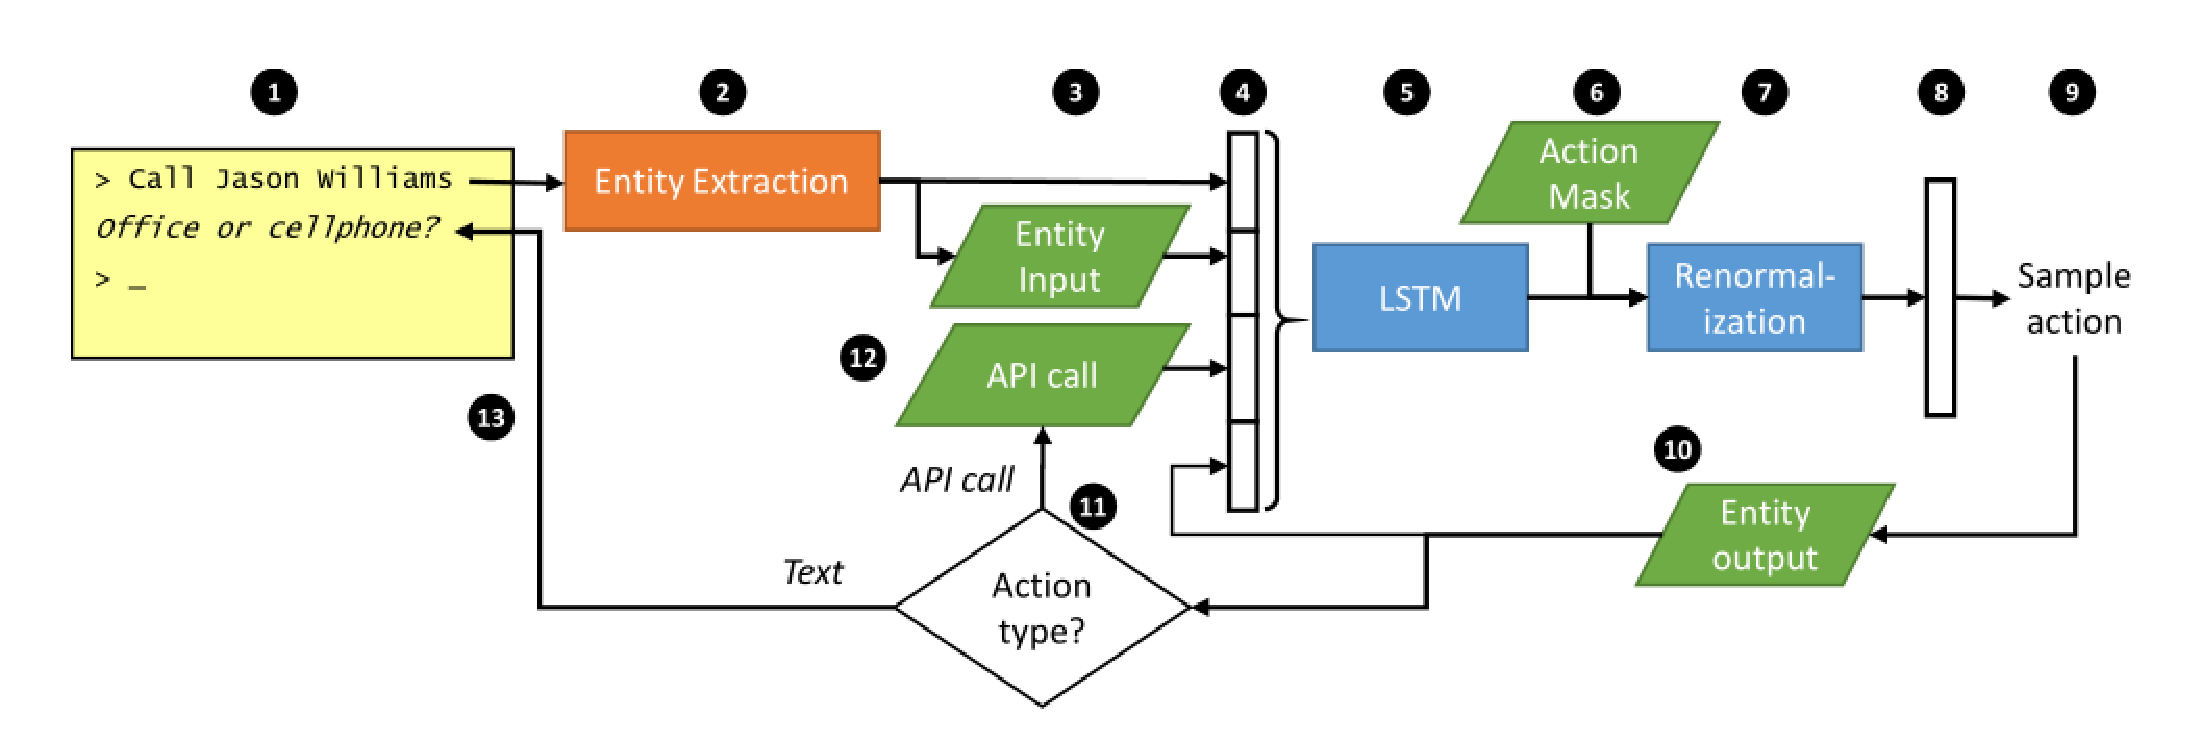
\includegraphics[width=\linewidth]{Williams2016End01}\\
  \caption{Operational loop of a dialogue system}\label{fig:Williams2016End01}
\end{figure}

The operational cycle has 13 steps: (1) The system receives user input; (2) The entities mentioned in user input are identified; (3) The extracted entities are resolved into ground entities corresponding to one or more rows in a database; (4) A feature vector is constructed from four sources; (5) LSTM takes the feature vector, update its hidden states, and outputs a distribution over all template actions; (6) Domain-specific software provides an action mask indicating actions that are not allowed at the current time; (7, 8) The task mask is combined with the distribution in step five into a new distribution; (9) An action is chosen from the new distribution; (10) The selected template action is instantiated with the entities in step three; (11, 12, 13) Depending on the action type, the system either invokes the corresponding API call or render the response text to users. 
\subsection{Learning End-to-End Goal-Oriented Dialog \cite{Bordes2016Learning}}

The main contributions of the paper are: (1) propose to evaluate end-to-end dialogue systems using goal-oriented tasks, and design five tasks in the application of restaurant reservation; (2) apply Memory Networks to train an end-to-end dialogue system, and show that per-response performance is encouraging.

The five tasks are (1) issue API calls. The system should ask questions, gather information about the preferred cuisine type, location, price range, and party size of restaurants, and generate the correct API call; (2) update API calls. When user preferences change, the system should update the API call; (3) display options. The system should propose the restaurants, which match user preferences, until users accept; (4) provide extra information. When users ask for the phone numbers and address of a restaurant, the system should answer correctly based on the facts; (5) conduct full dialogues (see Figure \ref{fig:Bordes2016Learning01} for examples of the five tasks). Natural language patterns and knowledge base entities are combined to generate simulated dialogues consisting of user and system utterances.

\begin{figure}[htbp]
  \centering
  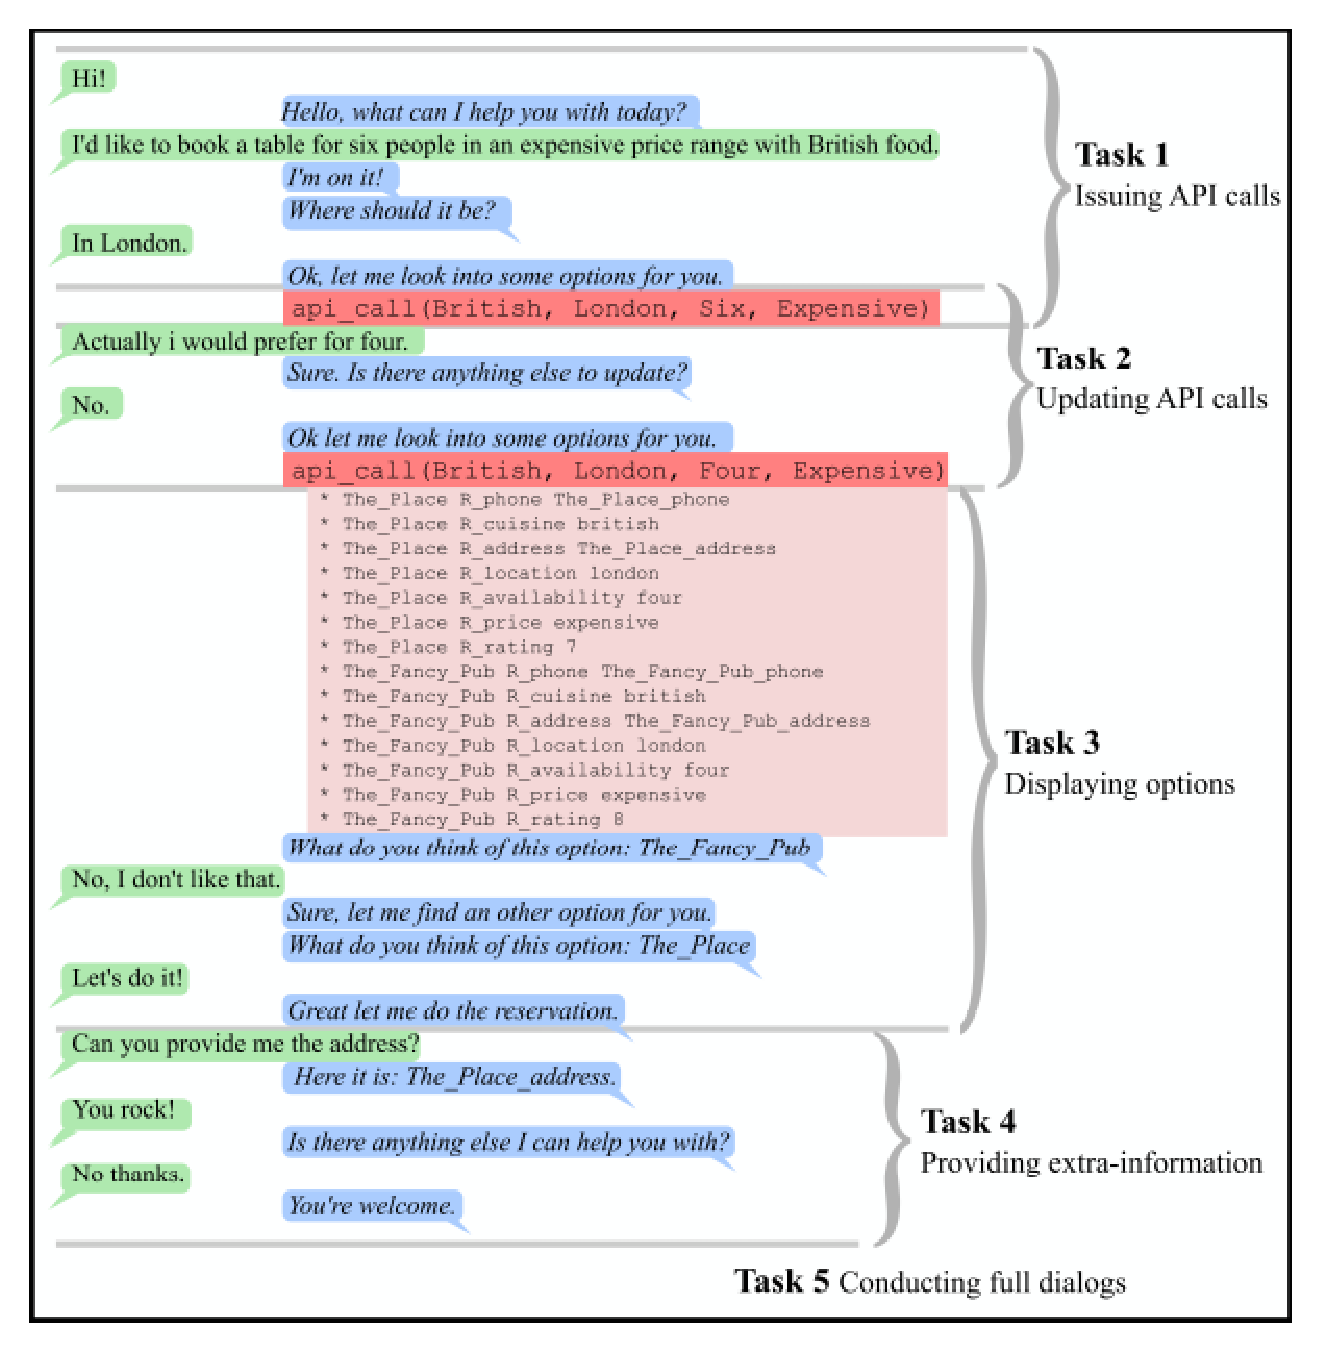
\includegraphics[width=.8\linewidth]{Bordes2016Learning01}\\
  \caption{Examples of the five tasks}\label{fig:Bordes2016Learning01}
\end{figure}

The paper uses a retrieval-based method, i.e. selecting the best candidate response from a large set of all possible system utterances and API calls. The paper applies Memory Networks that consist of three component (1) store conversation in memory; (2) read pertinent information from the memory; (3) use the information to output the best candidate response. 
\subsection{A Network-based End-to-End Trainable Task-oriented Dialogue System \cite{Wen2016}}
The task is to help humans find a desired restaurant and the contact information from a database by conversing naturally with them. The paper proposes an end-to-end trainable framework for task-oriented systems shown in Figure \ref{fig:Wen2016Network01}.

\begin{figure}[htbp]
  \centering
  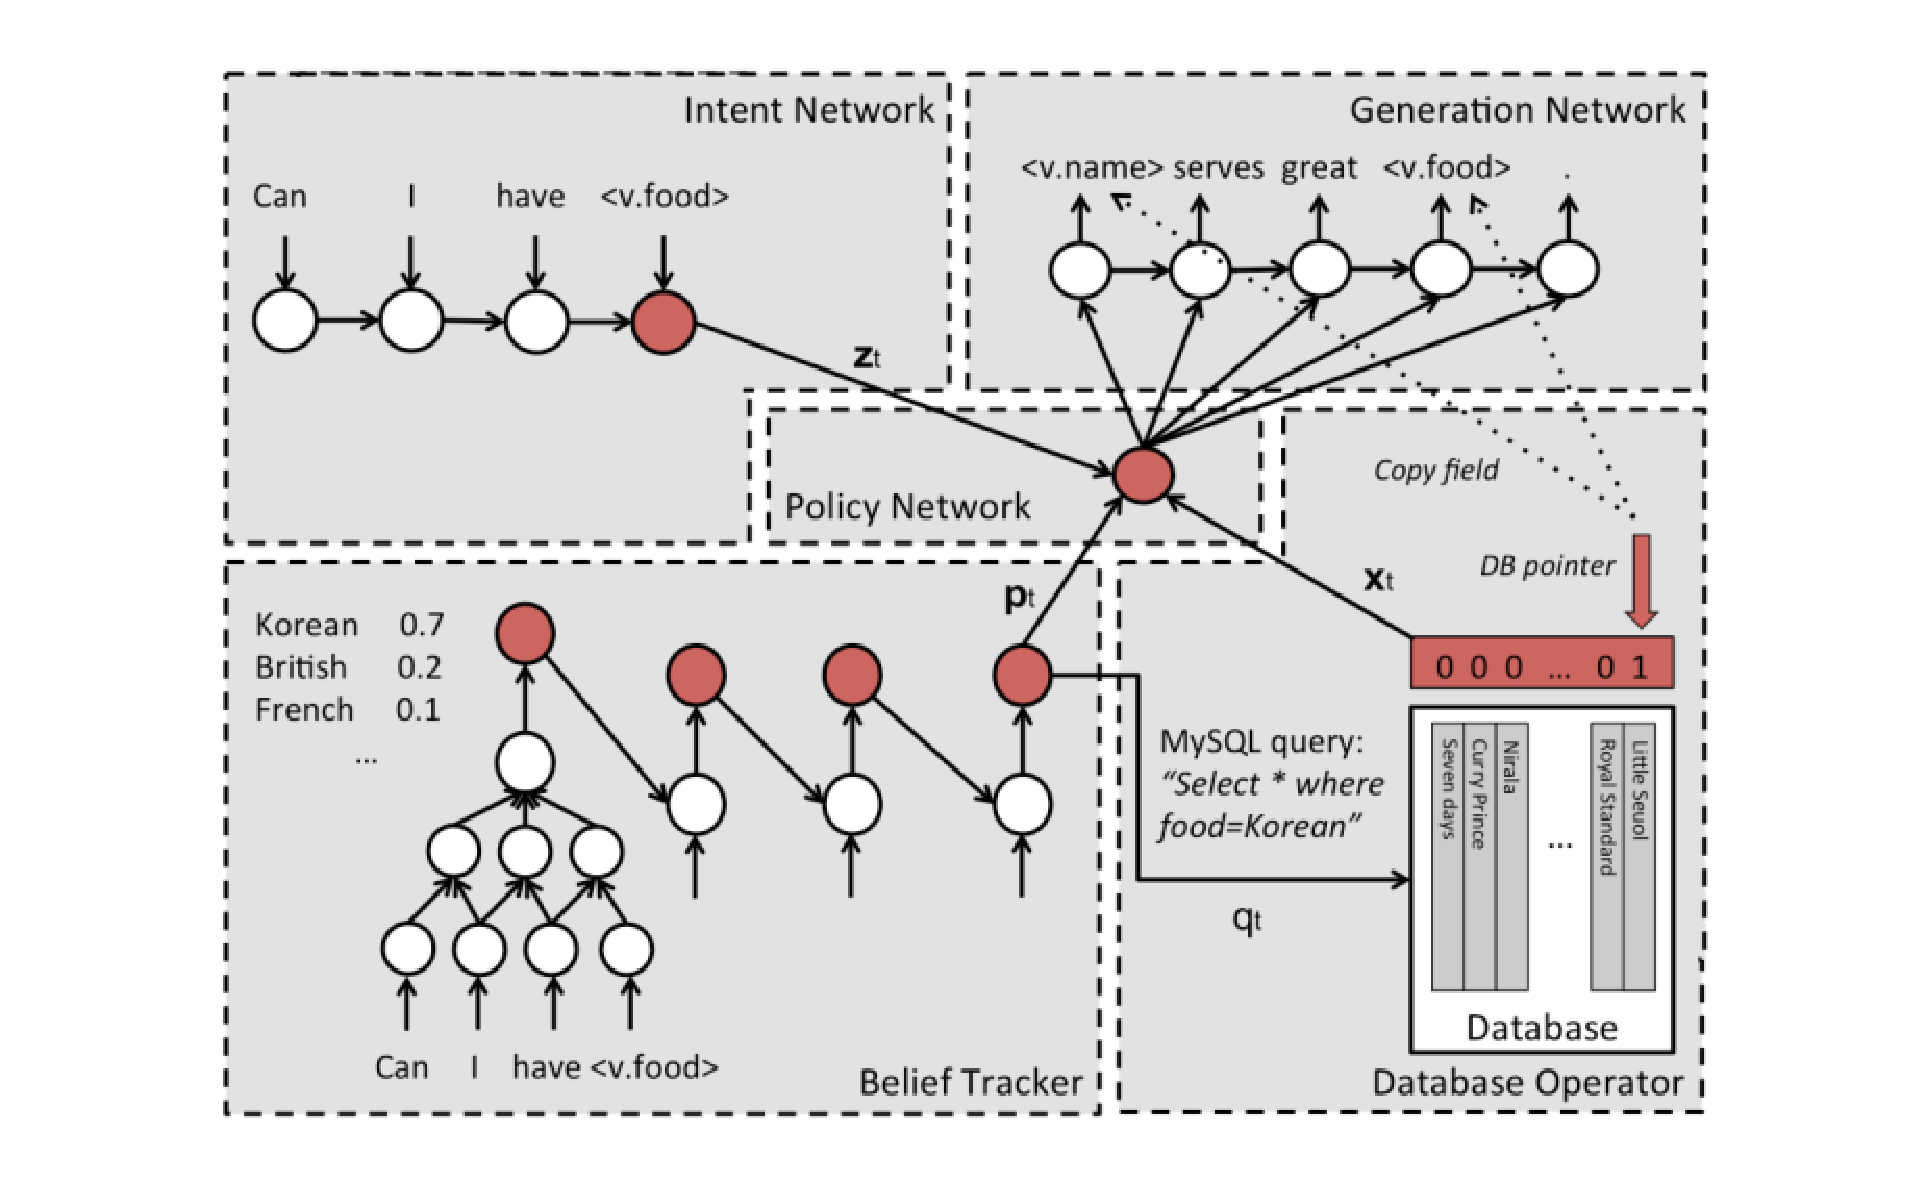
\includegraphics[width=0.9\linewidth]{Wen2016Network01}
  \caption{An end-to-end trainable framework for task-oriented systems}
	\label{fig:Wen2016Network01}
\end{figure}

At each turn, the system takes an user utterance $u^{t}$ as input, which is used to update two internal representations by an intent network and a set of belief trackers: (1) A distributed representation; (2) A distribution over the values, belief state, for each slot. The database operator uses the most likely values in the belief state, and returns the matched restaurants in the database. The policy network combines the distributed representation, belief state, and search results to form an action vector representing the next action. Conditioned on the action vector, the generation network produces template-like sentences whose generic tokens are then replaced by the actual values. Each components are described in more detail below:

\begin{itemize}
\item[-] \textbf{Intent Network} encodes $u^{t}=w^{t}_{0}, ..., w^{t}_{N}$ into a distributed representation $z^{t}$ at turn $t$. a LSTM is used and the last hidden state $z^{t}_{N}$ is taken as the distributed representation:
\begin{equation}
z^{t} \ = \ z^{t}_{N} \ = \ LSTM( w^{t}_{0}, ..., w^{t}_{N} )
\end{equation}

\item[-] \textbf{Belief Trackers} maintain a multinomial distribution $p^{t}_{s}$ for each informable slot and a bernoulli distribution $p^{t}_{s}$ for each requestable slot. The distributions are updated by:
\begin{equation}
\begin{aligned}
f^{t}_{s}(v) \ =& \ f^{t}_{s}(v,cnn) \oplus p^{t-1}_{s}(v) \oplus p^{t-1}_{s}(\emptyset) \\
g^{t}_{s}(v) \ =& \ U_{s} sigmoid( W_{s}f^{t}_{s}(v) + B_{s} ) + D_{s} \\
p^{t}_{s}(v) \ =& \ \frac{\exp(g^{t}_{s}(v))}{\exp(g^{t}_{s}(\emptyset)) + \sum_{v} \exp(g^{t}_{s}(v))} \\
\end{aligned}
\end{equation}
where $f^{t}_{s}(v)$ is the concatenation of two CNN feature vectors, one from processing $u^{t}$ and the other from processing the last action $a^{t-1}$.

\item[-] \textbf{Database Operator} forms a query
\begin{equation}
q^{t} \ = \ \cup_{s} { argmax_{v} p^{t}_{s}(v) }
\end{equation}
and create a binary vector $x^{t}$ over the restaurants in the database where a 1 means that the corresponding restaurant is consistent with the query.

\item[-] \textbf{Policy Network} outputs an action vector $o^{t}$ by:
\begin{equation}
o^{t} \ = \ \tanh( W_{z} z^{t} + W_{p} \oplus_{s} \hat{p}^{t}_{s} + W_{x} \hat{x}^{t} )
\end{equation}
where $\hat{p}^{t}_{s}$ is the belief summary consisting of (1) the summed value probabilities; (2) the probability that the user do not care; (3) the probability that the slot has not been mentioned, and $\hat{x}^{t}$ is a 6-bin 1-hot encoding vector based on the number of matched restaurants in $x^{t}$.

\item[-] \textbf{Generation Network} generates templates token by token conditioned on the action vector:
\begin{equation}
P(w^{t}_{i+1} | w^{t}_{i}, h^{t}_{i-1}, o^{t}) \ = \ LSTM( w^{t}_{i}, h^{t}_{i-1}, o^{t} )
\end{equation}
Instead of conditioning on a single action vector $o^{t}$, an attention mechanism can also be used to produce templates.

\end{itemize}
\subsection{Word-based dialog state tracking with recurrent neural networks \cite{Henderson2014Word}}

The task is to converts user inputs into dialogue states (see Table \ref{Goal-Oriented Dialogue System Example} for an example of dialogue state). The dialogue state is a probability distribution over handcrafted goals, methods, and requested slots. The paper uses a RNN to compute the distribution over goal values for each goal, a RNN to compute the distribution over methods, and a RNN to compute the distribution over requested slots. During training, gradient clipping is used to avoid exploding gradients \cite{Pascanu2012Understanding}.

\begin{table}[!hbp]
\begin{tabular}{|r|rl|}
\hline
\textbf{System Output} & \multicolumn{2}{l|}{You can ask for restaurants by area, price range or food type.} \\
\hline
\textbf{User Input} & \multicolumn{2}{l|}{Expensive restaurant in the south part of town.} \\
\hline
\emph{Dialogue State} & goals
& 0.7 pricerange=expensive area=south \\
&& 0.2 pricerange=expensive area=north \\
& methods & 0.9 method=byconstraints \\
&& 0.1 method=byalternatives \\
& requested slots & 0.0 address \\
&& 0.0 phone \\
\hline
\emph{System Act} & \multicolumn{2}{l|}{request(food)} \\
\hline
\textbf{System Output} & \multicolumn{2}{l|}{What kind of food would you like?} \\
\hline
\end{tabular}
\caption{Goal-Driven Dialogue System} \label{Goal-Oriented Dialogue System Example}
\end{table}
\subsection{End-to-End Reinforcement Learning of Dialogue Agents for Information Access \cite{Dhingra2016End}}
The task is to provide a user with an sorted list of entities, which are believed to match the user goal, from a database through dialogue. The paper presents an end-to-end trainable system: \emph{KB-InfoBot}. The high-level overview of KB-InfoBot is shown in Figure \ref{fig:Dhingra2016End01}.

\begin{figure}[htbp]
  \centering
  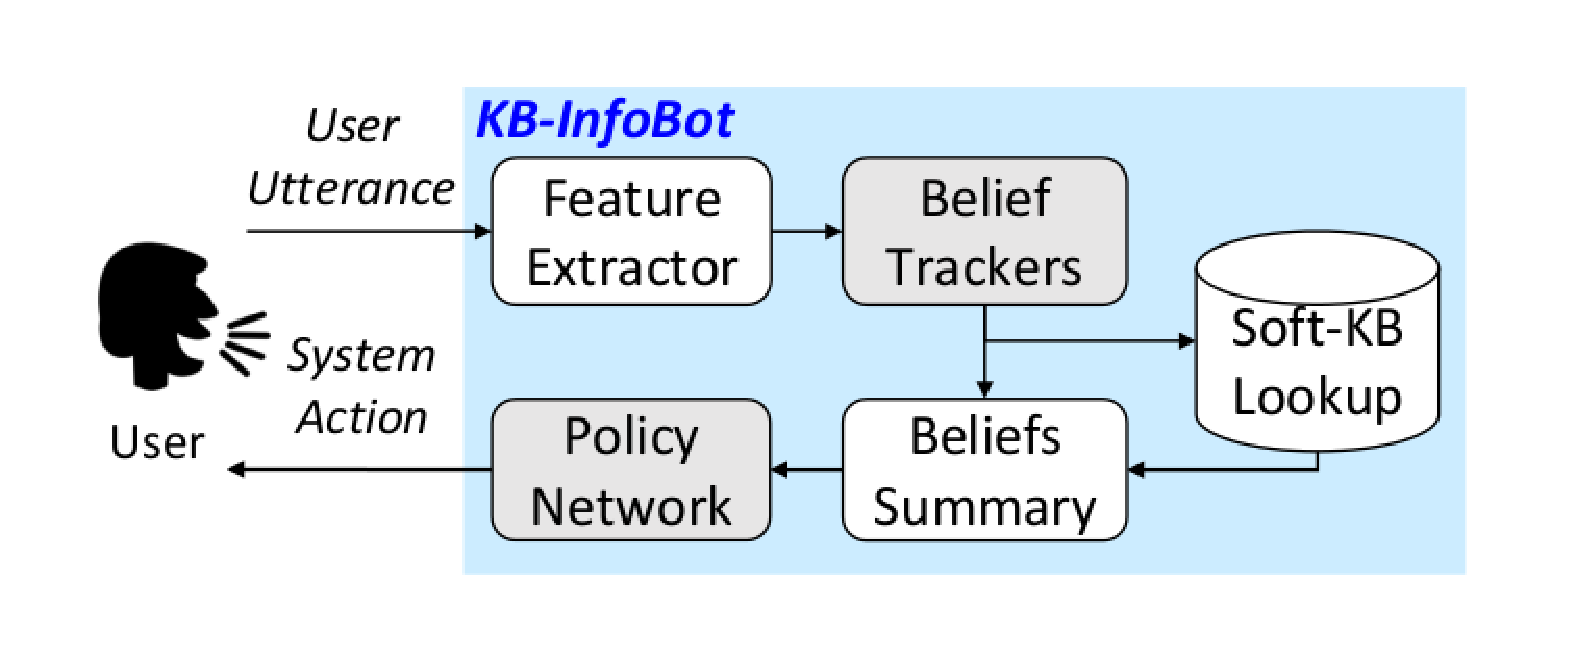
\includegraphics[width=0.8\linewidth]{Dhingra2016End01}
  \caption{KB-InfoBot}
	\label{fig:Dhingra2016End01}
\end{figure}

Assuming that in the database, there are $N$ entities, each of which has $M$ slots. At each turn, the input is an user utterance $u^{t}$ and the output is a system action $a^{t}$. The action space $\mathcal{A}$ has $M+1$ actions: (1) \emph{request($s_{j}$)} asking the user for the value of slot $j$ for $1 \leq j \leq M$; (2) \emph{inform($I$)} showing an sorted list of entities to the user. Each component of KB-InfoBot is defined as follows:

\begin{itemize}
\item[-] \textbf{Feature Extractor} converts $u^{t}$ into a vector representation $x^{t}$, each element of which indicates the count of a certain 2-gram in $u^{t}$. The vocabulary size is 3078 and thus $x^{t}$ is a 3078-dimensional vector.

\item[-] \textbf{Belief Tracker} takes $x^{t}$ as input and for each slot, updates the internal representation $h^{t}_{j}$ and outputs the belief state $p^{t}_{j}$ and $q^{t}_{j}$. The internal representation starting from $h^{0}_{j}=\mathbf{0}$ is updated by a Gated Recurrent Unit:
\begin{equation}
\begin{aligned}
r^{t}_{j} \ =& \ \sigma( W^{r}_{j}x^{t} + U^{r}_{j}h^{t-1}_{j} + b^{r} ) \\
z^{t}_{j} \ =& \ \sigma( W^{z}_{j}x^{t} + U^{z}_{j}h^{t-1}_{j} + b^{z} ) \\
h^{t}_{j} \ =& \ (1-z^{t}_{j}) \odot h^{t-1}_{j} + z^{t}_{j} \odot \tanh( W^{h}_{j}x^{t} + U^{h}_{j}(r^{t}_{j} \odot h^{t-1}_{j}) + b^{h} ) \\
\end{aligned}
\end{equation}
Then, the belief state is computed:
\begin{equation}
\begin{aligned}
p^{t}_{j} \ =& \ softmax( W^{p}_{j}h^{t}_{j} + b^{p}_{j} ) \\
q^{t}_{j} \ =& \ \sigma( W^{q}_{j}h^{t}_{j} + b^{q}_{j} ) \\
\end{aligned}
\end{equation}
where $p^{t}_{j}$ is a multinomial distribution over all the possible values of slot $j$, and $q^{t}_{j}$ is a bernoulli distribution indicating whether the user know the value of slot $j$ or not.

\item[-] \textbf{Soft-KB Lookup} uses $p^{t}_{j}$ and $q^{t}_{j}$ to compute $p^{t}$, the posterior distribution over the entities in the database:
\begin{equation}
p^{t}(i) \ \propto \ \prod_{j=1}^{M} p^{t}_{j} (i) \\
\end{equation}
which is the posterior probability that the $i$th entity is targeted by the user.
\[
    p^{t}_{j}(i) \ = \
\begin{cases}
    \frac{1}{N},                                                                                     & \text{if } i \in M_{j} \\
    q^{t}_{j}\frac{p^{t}_{j}(i_{j})}{N_{j}(i_{j})} (1- \frac{|M_{j}|}{N}) + (1-q^{t}_{j})\frac{1}{N},& \text{otherwise}
\end{cases}
\]
where $N_{j}(i_{j})$ is the count of value $i_{j}$ in slot $j$, and $M_{j}$ is the set of entities for which the value of slot $j$ is missing.

\item[-] \textbf{Beliefs Summary} summarizes slot $j$ into an entropy statistic, $H(p^{t}_{j})$, over a distribution $w^{t}_{j}$:
\begin{equation}
w^{t}_{j}(v) \ \propto \ \sum_{i:i_{j}=v} p^{t}(i) + p^{0}_{j}(v) \sum_{i:i_{j}\ is\ missing} p^{t}(i) \\
\end{equation}
In a similar way, $p^{t}$ is summarized into $H(p^{t})$. The summary vector $s^{t}=[H(p^{t}_{1}), ..., H(p^{t}_{M}), q^{t}_{1}, ..., q^{t}_{M}, H(p^{t})]$ is input to the policy network.

\item[-] \textbf{Policy Network} selects the next action based on the dialogue history and the current summary vector $s^{t}$:
\begin{equation}
\begin{aligned}
h^{t}_{\pi} \ =& \ GRU( s^{1}, ..., s^{t} ) \\
\pi \ =& \ softmax( W^{\pi}h^{t}_{\pi} + b^{\pi} ) \\
\end{aligned}
\end{equation}

\item[-] \textbf{Action Selection} samples the next action from the polity $\pi$. If action \emph{inform()} is chosen, an ordered list $I=(i_{1}, ..., i_{R})$ of indices is provided to the user.
\end{itemize}
